\section{Introducción}
En este T.P. deberemos decidir si la estructura de un puente, con ciertas cargas dadas, es estable. En este caso, analizaremos la estructura de puentes \emph{Prat Truss}, escribiendo las ecuaciones de fuerzas que se aplican sobre ciertas partes de la estructura. Luego resolveremos este sistema lineal y verificaremos que ninguna de los valores de fuerza obtenidos superen un límite determinado por los materiales de construcción. Para resolver el sistema utilizaremos el método de Eliminación de Gauss, al que aplicaremos algunas optimizaciones que permite este problema en particular, al igual que para la representación de la matriz en memoria. 

Una vez que contemos con una manera eficiente de determinar las fuerzas que actúan sobre el puente dada una cierta configuración de cargas, consideraremos colocar pilares intermedios de concreto si alguna fuerza pusiera en peligro la seguridad del puente. Para esto, desarrollaremos una heurística que decida cuántos y dónde ubicarlos para minimizar el costo de construcción, dado que la inserción de estos pilares es altamente costosa.

\subsection{Puentes \emph{Pratt Truss}}
Un esquema de puente \emph{Pratt Truss} puede verse en la figura \ref{fig:puente}.
\begin{figure}[!ht]
\begin{center}
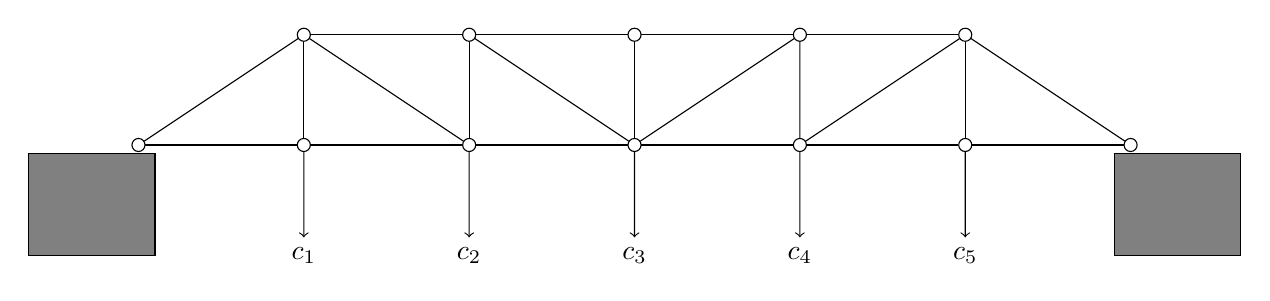
\begin{tikzpicture}[scale = 0.7]

    \tikzset{nodestyle/.style={draw,shape=circle,scale=0.5}}
    \node[nodestyle] (p1) at ( 0, 0) {}; 
    \node[nodestyle] (p2) at ( 3, 0) {};
    \node[nodestyle] (p3) at ( 6, 0) {};
    \node[nodestyle] (p4) at ( 9, 0) {};
    \node[nodestyle] (p5) at ( 12, 0) {};
    \node[nodestyle] (p6) at ( 15, 0) {};
    \node[nodestyle] (p7) at ( 18, 0) {};

    \node[nodestyle] (p8) at ( 3, 2) {};
    \node[nodestyle] (p9) at ( 6, 2) {};
    \node[nodestyle] (p10) at ( 9, 2) {};
    \node[nodestyle] (p11) at ( 12, 2) {};
    \node[nodestyle] (p12) at ( 15, 2) {};

    \begin{scope}[every path/.style={-}]
        \draw (p1) -- (p2);
        \draw (p2) -- (p3); 
        \draw (p3) -- (p4);
        \draw (p4) -- (p5);
        \draw (p5) -- (p6);
        \draw (p6) -- (p7);

        \draw (p8) -- (p9);
        \draw (p9) -- (p10);
        \draw (p10) -- (p11);
        \draw (p11) -- (p12);

        \draw (p1) -- (p8);
        \draw (p12) -- (p7);

        \draw (p2) -- (p8);
        \draw (p3) -- (p9);
        \draw (p4) -- (p10);
        \draw (p5) -- (p11);
        \draw (p6) -- (p12);

        \draw (p8) -- (p3);
        \draw (p9) -- (p4);
        \draw (p4) -- (p11);
        \draw (p5) -- (p12);
    \end{scope}  

        \draw[fill=gray] (0.3,-0.15) rectangle (-2,-2);
        \draw[fill=gray] (17.7,-0.15) rectangle (20,-2);

    \node (c1) at ( 3, -2) {$c_1$};
    \node (c2) at ( 6, -2) {$c_2$};
    \node (c3) at ( 9, -2) {$c_3$};
    \node (c4) at ( 12, -2) {$c_4$};
    \node (c5) at ( 15, -2) {$c_5$};
    \draw[->] (p2) -- (c1);
  	\draw[->] (p3) -- (c2);
   	\draw[->] (p4) -- (c3);
    \draw[->] (p5) -- (c4);
    \draw[->] (p6) -- (c5);
\end{tikzpicture}
\caption{Esquema de la estructura de un puente \emph{Pratt Truss}. \small{(Cortesía Enunciado TP2)}}
\label{fig:puente}
\end{center}
\end{figure}

Dado que realizaremos el análisis únicamente en dos dimensiones (supondremos que las cargas se distribuyen uniformemente en la profundidad), pensaremos de ahora en más en esquemas como éste. Llamaremos \emph{link} a cada uno de los miembros de los que se compone la estructura, \emph{junta} a los puntos donde éstos se unen y \emph{sección} a la porción contenida entre dos links verticales sucesivos. Para el análisis en el T.P. trabajaremos con una cantidad par de secciones y supondremos que las cargas (y las fuerzas en general) se aplican únicamente sobre las juntas. Consideraremos como variables de la estructura la cantidad de secciones ($n$), la altura del puente ($h$), y la luz que debe cubrir ($span$). Podemos ver (como se muestraen la figura \ref{fig:estructuras}) que una estructura de $n$ secciones cuenta con $2n$ juntas y $4n-3$ links.

\begin{figure}[!ht]
\begin{center}
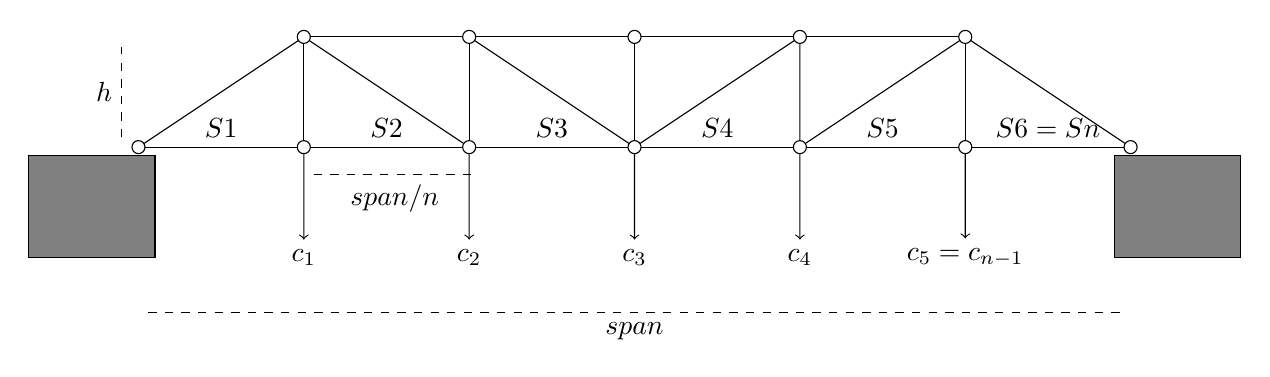
\begin{tikzpicture}[scale = 0.7]

    \tikzset{nodestyle/.style={draw,shape=circle,scale=0.5}}
    \node[nodestyle] (p1) at ( 0, 0) {}; 
    \node[nodestyle] (p2) at ( 3, 0) {};
    \node[nodestyle] (p3) at ( 6, 0) {};
    \node[nodestyle] (p4) at ( 9, 0) {};
    \node[nodestyle] (p5) at ( 12, 0) {};
    \node[nodestyle] (p6) at ( 15, 0) {};
    \node[nodestyle] (p7) at ( 18, 0) {};

    \node[nodestyle] (p8) at ( 3, 2) {};
    \node[nodestyle] (p9) at ( 6, 2) {};
    \node[nodestyle] (p10) at ( 9, 2) {};
    \node[nodestyle] (p11) at ( 12, 2) {};
    \node[nodestyle] (p12) at ( 15, 2) {};

    \begin{scope}[every path/.style={-}]
        \draw (p1) -- (p2) node[midway,above] {$S1$};
        \draw (p2) -- (p3) node[midway,above] {$S2$}; 
        \draw (p3) -- (p4) node[midway,above] {$S3$};
        \draw (p4) -- (p5) node[midway,above] {$S4$};
        \draw (p5) -- (p6) node[midway,above] {$S5$};
        \draw (p6) -- (p7) node[midway,above] {$S6= Sn$};

        \draw (p8) -- (p9);
        \draw (p9) -- (p10);
        \draw (p10) -- (p11);
        \draw (p11) -- (p12);

        \draw (p1) -- (p8);
        \draw (p12) -- (p7);

        \draw (p2) -- (p8);
        \draw (p3) -- (p9);
        \draw (p4) -- (p10);
        \draw (p5) -- (p11);
        \draw (p6) -- (p12);

        \draw (p8) -- (p3);
        \draw (p9) -- (p4);
        \draw (p4) -- (p11);
        \draw (p5) -- (p12);
    \end{scope}  

        \draw[fill=gray] (0.3,-0.15) rectangle (-2,-2);
        \draw[fill=gray] (17.7,-0.15) rectangle (20,-2);

        % Nodos artificiales.
        \node (a1) at ( 0, -3) {};
        \node (a2) at ( 18, -3) {};
        \node (a3) at ( -0.3, 0) {};
        \node (a4) at ( -0.3, 2) {};
        \node (a5) at ( 3, -0.5) {};
        \node (a6) at ( 6.3, -0.5) {};
		\node (c1) at ( 3, -2) {$c_1$};
    \node (c2) at ( 6, -2) {$c_2$};
    \node (c3) at ( 9, -2) {$c_3$};
    \node (c4) at ( 12, -2) {$c_4$};
    \node (c5) at ( 15, -2) {$c_5  = c_{n-1}$};
    \draw[->] (p2) -- (c1);
  	\draw[->] (p3) -- (c2);
   	\draw[->] (p4) -- (c3);
    \draw[->] (p5) -- (c4);
    \draw[->] (p6) -- (c5);        
        
        
        \begin{scope}[every path/.style={-}]
            \draw[dashed] (a1) -- (a2) node[below,midway]{$span$} ;
            \draw[dashed] (a3) -- (a4) node[left,midway]{$h$};
            \draw[dashed] (a5) -- (a6) node[below,midway]{$span/n$};
        \end{scope}
        
\end{tikzpicture}
\caption{Variables a considerar de la estructura, $n = 6$. \small{(Cortesía Enunciado TP2)}}
\label{fig:estructuras}
\end{center}
\end{figure}


Para asegurar la estabilidad, requeriremos que la fuerza resultante sobre cada junta sea nula. Es decir, que las fuerzas horizontales y verticales (y la descomposición en estas direcciones de las fuerzas oblicuas) se anulen en cada junta. Para satisfacer esto, consideraremos, por cada junta, una ecuación en dirección horizontal y otra en vertical, cuyas incógnitas serán las fuerzas ejercidads por los links. Construyendo esto para todas las juntas, tendremos un sistema de $4n$ ecuaciones. Si consideramos una variable por la fuerza ejercida por cada link tendremos $4n-3$ variables, a las que agregaremos fuerzas verticales sobre las juntas de los extremos y una fuerza horizontal sobre uno de éstos, para modelar la interacción del terreno, tendremos un sistema cuadrado de $4n$. Observemos que la cantidad de fuerzas que se ejercen sobre cada link es una cantidad constante (y pequeña) en relación al tamaño de la estructura, con lo cual, la mayoría de los coeficientes de las incógnitas serán nulos, generando una 
matriz muy esparsa.

\subsection{Representación Matricial}
Dado que las variables involucradas en cada ecuación son pocas, la matriz asociada al sistema resulta con una gran cantidad de coeficientes nulos, lo que nos motivó a utilizar una estructura de datos que aproveche este hecho, antes que la implementación trivial como arreglo bidimensional. Más aún, veremos que la matriz resultante tiene estructura de bandas, y que nuestro algoritmo de eliminación la conserva, con lo cual durante toda la vida de la matriz, sigue siendo considerablemente esparsa, con lo cual las ventajas siguen siendo válidas. En esta representación, decidimos almacenar las filas como listas enlazadas ordenadas por índice creciente, conteniendo únicamente elementos no nulos. La matriz, entonces, resulta en un vector de $n$ filas, en la cual, si bien el acceso aleatorio al elemento $i,j$ es más costoso que en el caso del arreglo bidimensional, las operaciones por filas tienen el mismo costo que en aquél y evitan considerar operaciones entre valores nulos.

\subsubsection{Matriz Banda}
Formalmente, decimos que una matriz $A \in \R ^{n\times n}$ tiene estructura de bandas $p,q$ si $a_{i,j} = 0$ cuando $j \leq i-p$ ó $j\geq i+q$, $1\leq i,j \leq n$.

\begin{lema}
Sea $A \in \R^{n \times n}$, con estructura de bandas $p, q$. Luego, en el peor de los casos, en todos los pasos del algoritmo de Eliminación Gaussiana con pivoteo parcial, la matriz resultante tiene estructura de bandas $p, q+p$
\end{lema}
\begin{proof}
Demostraremos el lema por inducción en la cantidad de pasos del algoritmo de eliminación gaussiana. \\
Sea $k$ = 1 el primer paso de la eliminación gaussiana. \\

Sea $a_{ij}$ = $\smash{\displaystyle\max_{1 \leq i \leq n}} |a_{i1}|$. Como $A$ es matriz banda $p, q$, $i \leq p$. \\

Por otro lado, a lo sumo el último elemento no nulo de la fila $i$ es el $a_{ii+q}$ (llamémoslo $a_{ij}$). Entonces, $j \leq q+i \leq q+p$ (pues $i \le p$). \\
Luego, al permutar la fila $k$ con la fila $i$, tenemos que el último elemento no nulo de la fila $k$ (ya permutada) está a distancia $\leq q+p$ por encima de la diagonal. Además, tras aplicar Gauss sólo se modifican $p-1$ filas, con lo cual la matriz resultante tiene banda inferior $\leq p$ y por lo dicho anteriormente, banda superior $\leq q+p$ ya que para las $p-1$ filas modificadas el último el elemento no nulo está, a lo sumo, en la columna $q+p$ (a distancia $q+p-i$ de la diagonal siendo $i$ la fila modificada) con lo cual la banda superior está dada por la fila $k$. \\

Hipótesis inductiva: Luego del paso k-ésimo del algoritmo de eliminación gaussiana (con $k < n$), la matriz resultante posee una estructura de bandas $p', q'$ ($p' \leq p, q' \leq q+p$).\\

Paso inductivo: Apliquemos el paso $k+1$. Del paso anterior obtuvimos, en el peor caso, una matriz banda $p, q+p$ por hipótesis inductiva. Además, sabemos que ninguna de las filas $i \geq p+k$ fue modificada en el paso anterior, pues el elemento $a_{ik}$ es nulo. Luego, si consideramos la submatriz $A'$ de dimensión $k+1 \times k+1$, tenemos que $A'$ es una matriz banda $p, q$ y entonces, aplicando el mismo razonamiento que para $k=1$, al aplicar Gauss obtendremos en el peor caso una matriz con bandas $p, q+p$.
\end{proof}

\subsection{Algoritmo de Resolución}
Como dijimos, utilizaremos el método de Eliminación de Gauss, al que le agregaremos pivoteo parcial  ya que no podemos asegurar que éste no sea necesario en las condiciones de la matriz. Más allá de esto, no realizamos mayores modificaciones al algoritmo, únicamente aprovechar la existencia de la banda inferior para reducir el alcance de la búsqueda del pivote, ya que por debajo de ésta sólo encontraría ceros.




